% !TeX encoding=unicode
% !TeX spellcheck = de-DE

\chapter{Results}
%
\section{Grid validiation}
In the following we will validate the interpolation method used by \mcgrid{} for the processes $pp \rightarrow H + (0,1,2) \text{jets}$ at the \SI{13}{\tera\electronvolt} LHC, computed at NLO.
Thereto, we generate reference distributions for different observables using the \sherpa{} event generator and compare them to the distributions obtained by convoluting a grid with the respective PDF.
Additionally, the results from \appl{} and \fnlo{} are compared to each other.
All grids are filled using the central value of the CT10 pdf set \cite{ct10}.
The examined observables are the transverse momenta $p_\perp$ of the Higgs boson and the $\tau$ leptons, respectively, the rapidity $y$ of the Higgs boson and the pseudorapidity $\eta$ of the $\tau$ leptons.
The projection of the observables into histogram bins is accomplished by the \rivet{} analysis system.
Final state jets are extracted by the \fastjet{} library \cite{fastjet_manual} using the anti-$k_t$ algorithm \cite{anti_kt} with a radius parameter $R=0.4$ and a $p_\perp$-cut of $p_\perp > \SI{20}{\giga\electronvolt}$.

The first validity test will check whether the grids are able to reproduce the distributions when they are filled with the same events as the reference histograms, i.e.\ when no parameter variation is performed.
This will also determine the interpolation accuracy.
Subsequently, the cases where the scale factors and/or PDFs of the grids are changed \textit{a posteriori} will be compared to reference distributions where these parameters have been set explicitly.
%
\subsection{Interpolation accuracy}
In this section we will prove, that the grids are able to reproduce the reference distributions up to the available interpolation accuracy.
For each observable, one high precision grid and one lower precision grid is used.
In the 0- and 1-jet cases, the high precision grid has \num{50} bins in $x$ and the lower precision grid has \num{30} bins in $x$.
In the 2-jet case, the high precision grid has \num{70} bins and the lower precision one has \num{50} bins.
This is because with higher jet multiplicity, the influence of high $x$ values increases while in all cases the same transformation is used to smooth the distribution.
As we have seen in \textcolor{red}{???????????????????????????????}, this transformation favors low values of $x$, so a relatively high number of grid points is needed to accurately represent the high $x$ region.
For all the following calculations, the scale parameters have been fixed to the mass of the Higgs boson.
Therefore, $Q^2$ does not change and only one bin is used.
To achieve better comparability, \appl{} is configured to use fourth order interpolation, which is the same as is hardcoded into the \fnlo{} library.
A sample of \num{1} million events is used to fill the grids.

\Cref{fig:hnlo_validation} shows the ratio of the results obtained by convoluting the grids with the CT10 PDF to the reference distributions for the 0-jet process.
Using the high precision grid, almost all bins show errors below \SI{0.1}{\percent}.
\appl{} and \fnlo{} show roughly the same accuracy but the lepton $p_\perp$ shows a few outliers with \fnlo{}.
The effect of using a smaller grid is considerably bigger for the $p_\perp$ distributions than for the rapidity distributions.
It is also bigger for \appl{} than for \fnlo{}.

With one jet (\cref{fig:hjnlo_validation}), the errors in the reproduction of the $p_\perp$ become notably larger, especially when using \fnlo{}.
There are comparatively large outliers using the lower precision grids.
Nonetheless, with the high precision grids the errors are still within \SI{0.3}{\percent}.

The case of two jets is shown in \cref{fig:hjjnlo_validation}.
Here the grid with \num{50} bins produces relatively large errors.
Though the plot does not comprise this, the highest errors are at the order of one percent.
However \textcolor{red}{\ldots}



%
\begin{sidewaysfigure}
\centering
\begin{subfigure}[]{0.49\textwidth}
	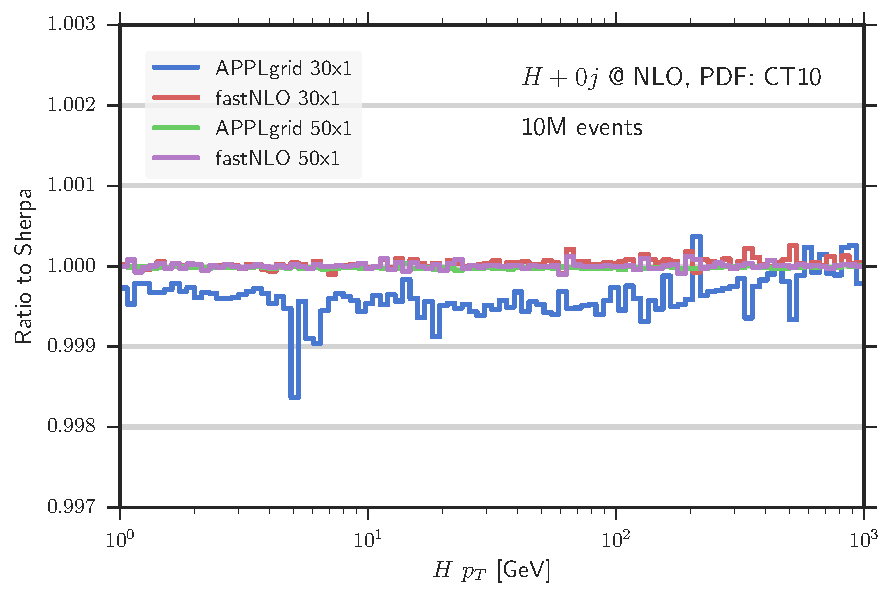
\includegraphics[width=\textwidth]{images/hnlo_hpt_50v30.pdf}
\end{subfigure}
\hfill
\begin{subfigure}[]{0.49\textwidth}
	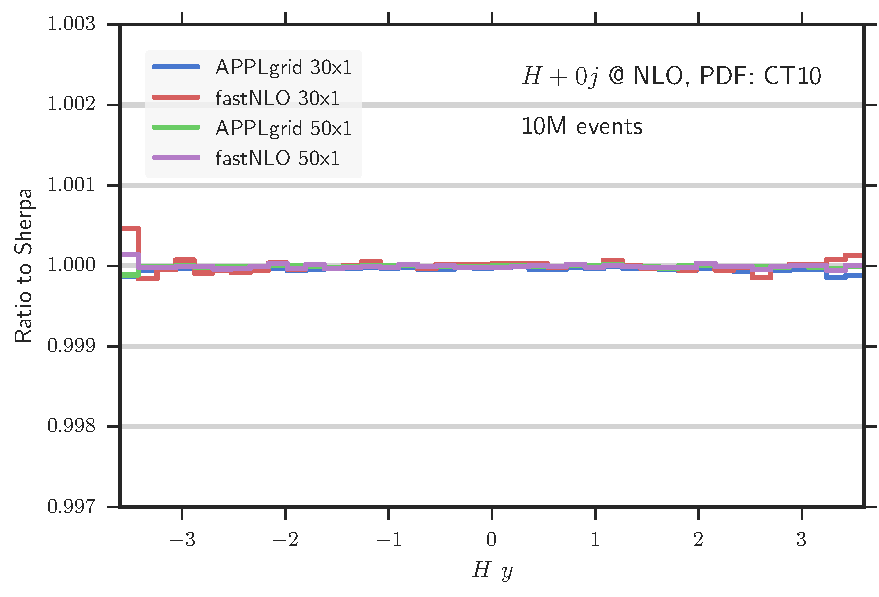
\includegraphics[width=\textwidth]{images/hnlo_hy_50v30.pdf}
\end{subfigure}

\begin{subfigure}[]{0.49\textwidth}
	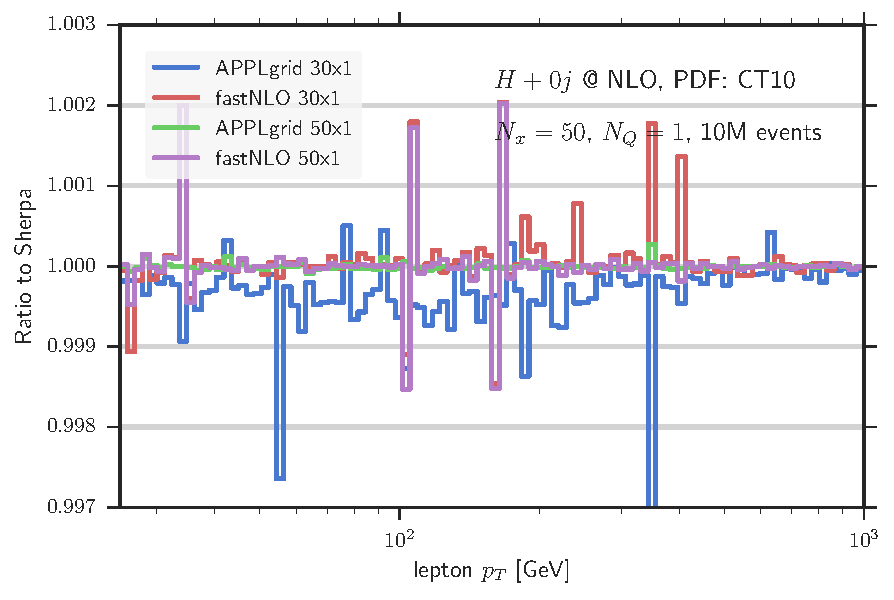
\includegraphics[width=\textwidth]{images/hnlo_lpt_50v30.pdf}
\end{subfigure}
\hfill
\begin{subfigure}[]{0.49\textwidth}
	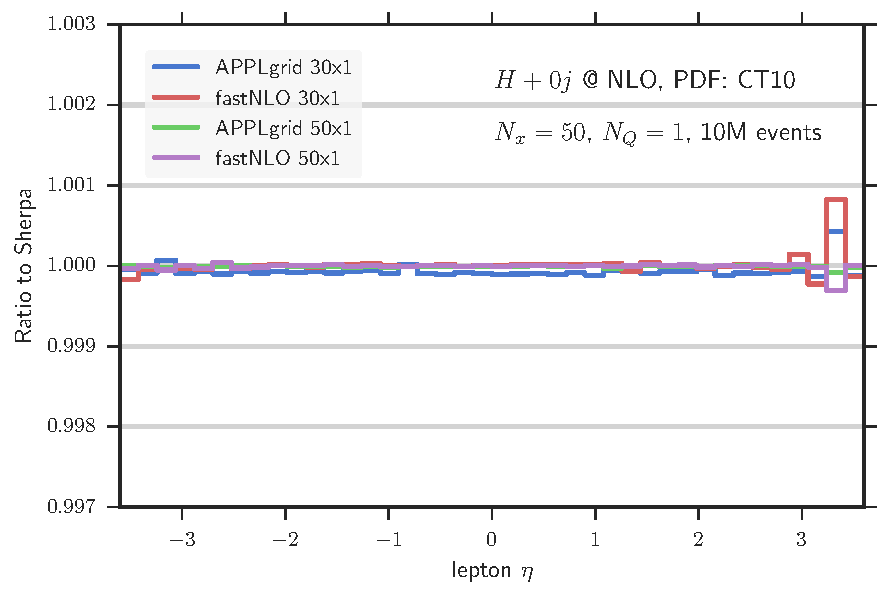
\includegraphics[width=\textwidth]{images/hnlo_leta_50v30.pdf}
\end{subfigure}
\caption{H+0j NLO}
\label{fig:hnlo_validation}
\end{sidewaysfigure}
%
\begin{sidewaysfigure}
\centering
\begin{subfigure}[]{0.49\textwidth}
	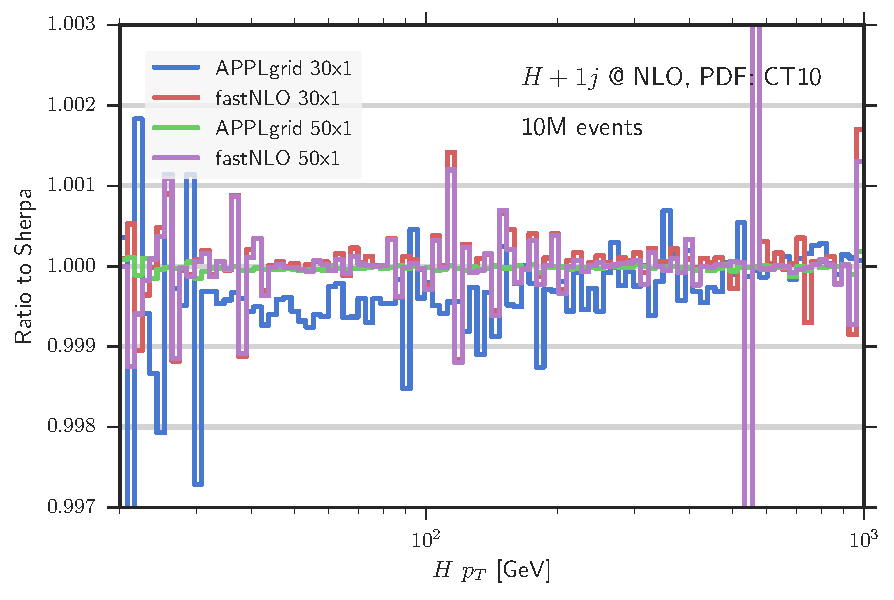
\includegraphics[width=\textwidth]{images/hjnlo_hpt_50v30.pdf}
\end{subfigure}
\hfill
\begin{subfigure}[]{0.49\textwidth}
	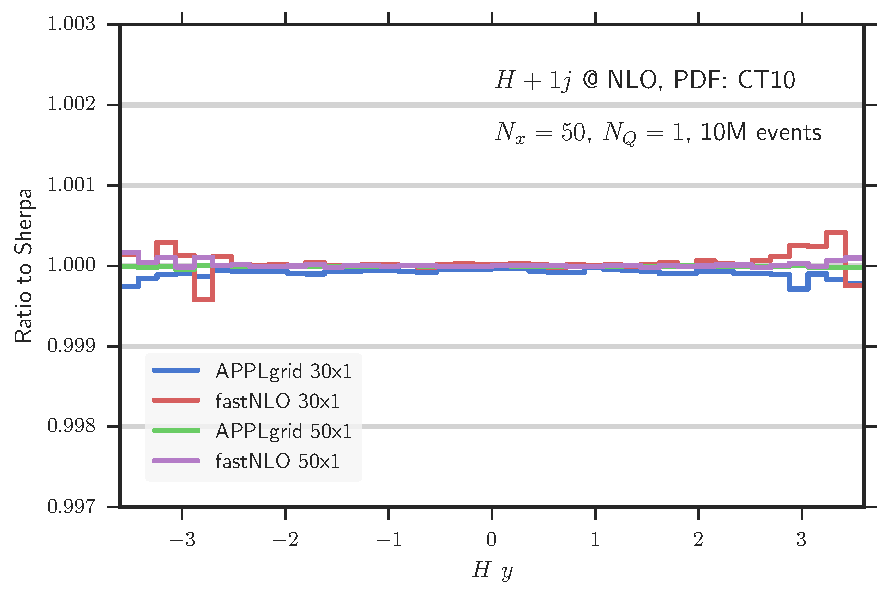
\includegraphics[width=\textwidth]{images/hjnlo_hy_50v30.pdf}
\end{subfigure}

\begin{subfigure}[]{0.49\textwidth}
	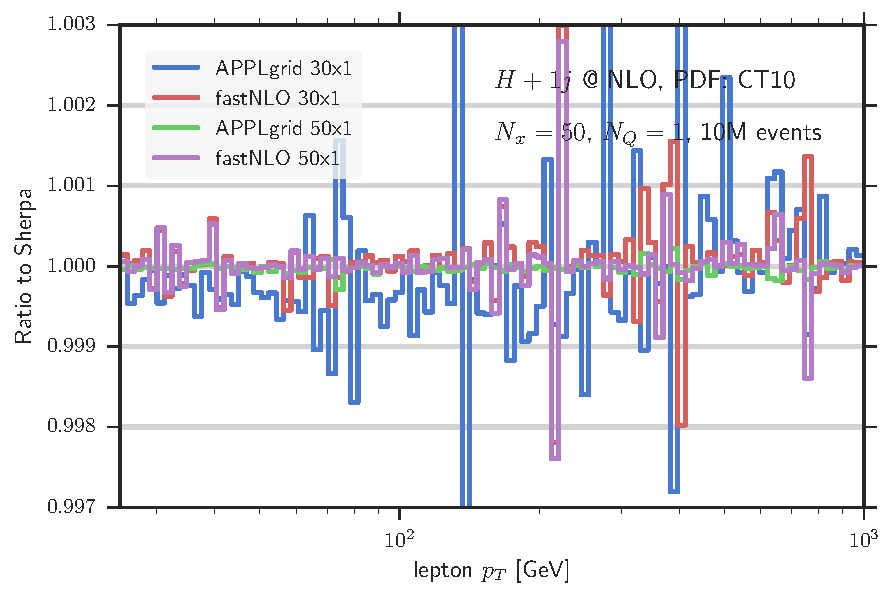
\includegraphics[width=\textwidth]{images/hjnlo_lpt_50v30.pdf}
\end{subfigure}
\hfill
\begin{subfigure}[]{0.49\textwidth}
	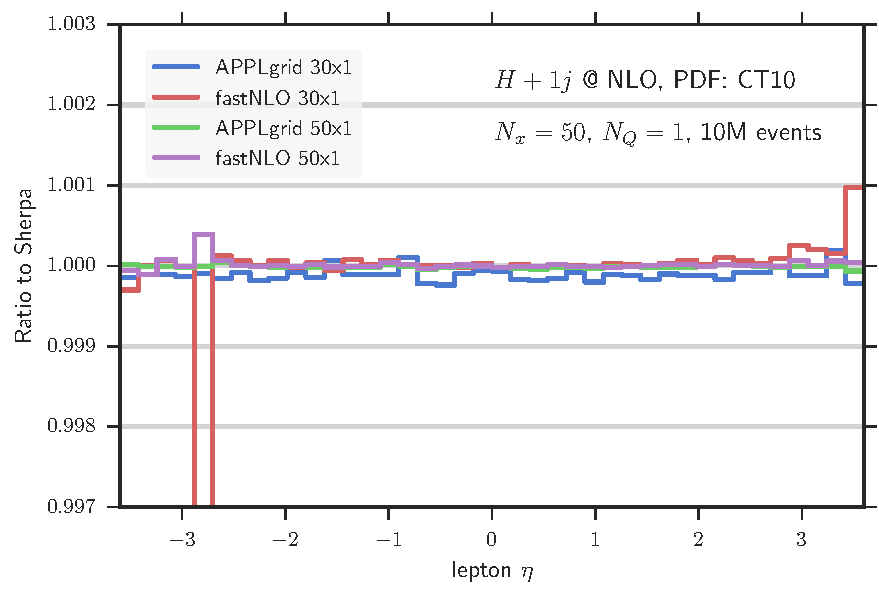
\includegraphics[width=\textwidth]{images/hjnlo_leta_50v30.pdf}
\end{subfigure}
\caption{H+1j NLO}
\label{fig:hjnlo_validation}
\end{sidewaysfigure}
%
\begin{sidewaysfigure}
\centering
\begin{subfigure}[]{0.49\textwidth}
	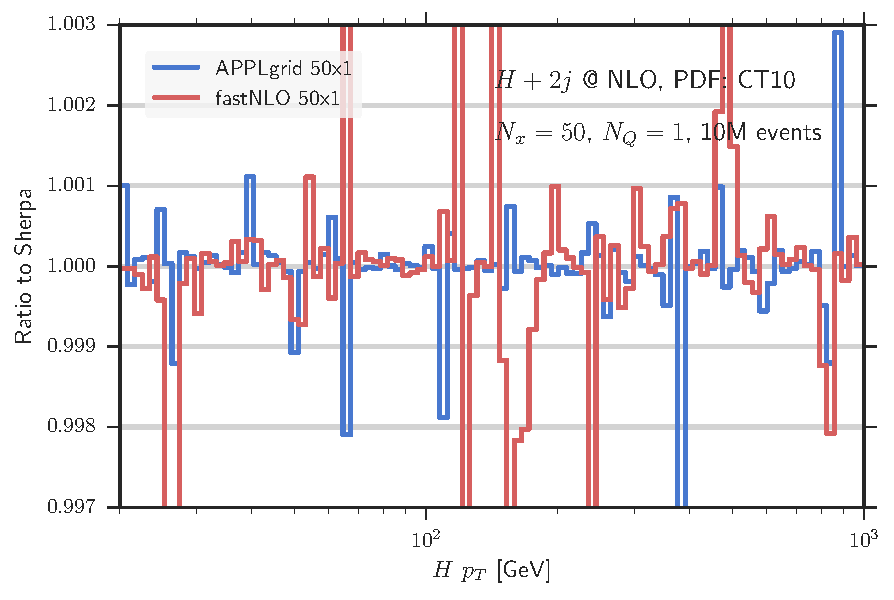
\includegraphics[width=\textwidth]{images/hjjnlo_hpt_50v30.pdf}
\end{subfigure}
\hfill
\begin{subfigure}[]{0.49\textwidth}
	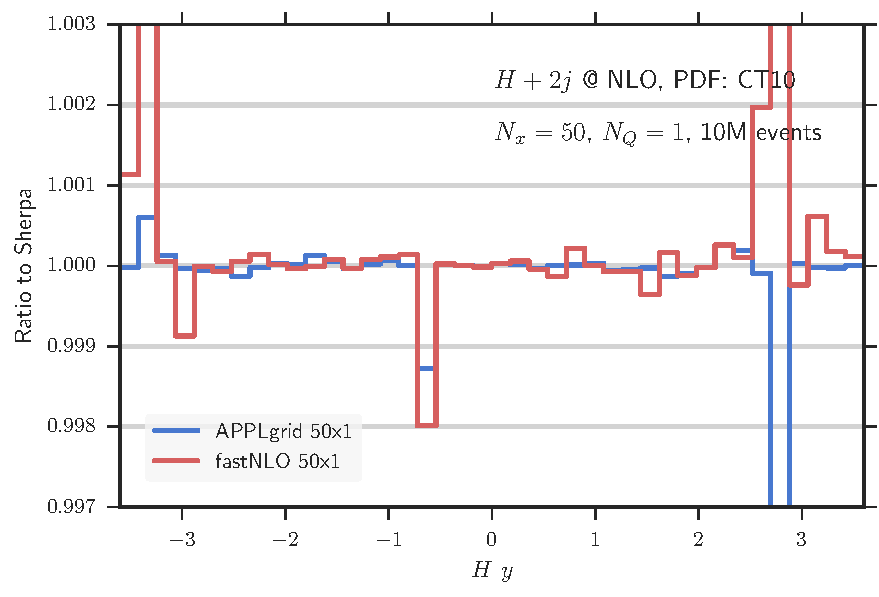
\includegraphics[width=\textwidth]{images/hjjnlo_hy_50v30.pdf}
\end{subfigure}

\begin{subfigure}[]{0.49\textwidth}
	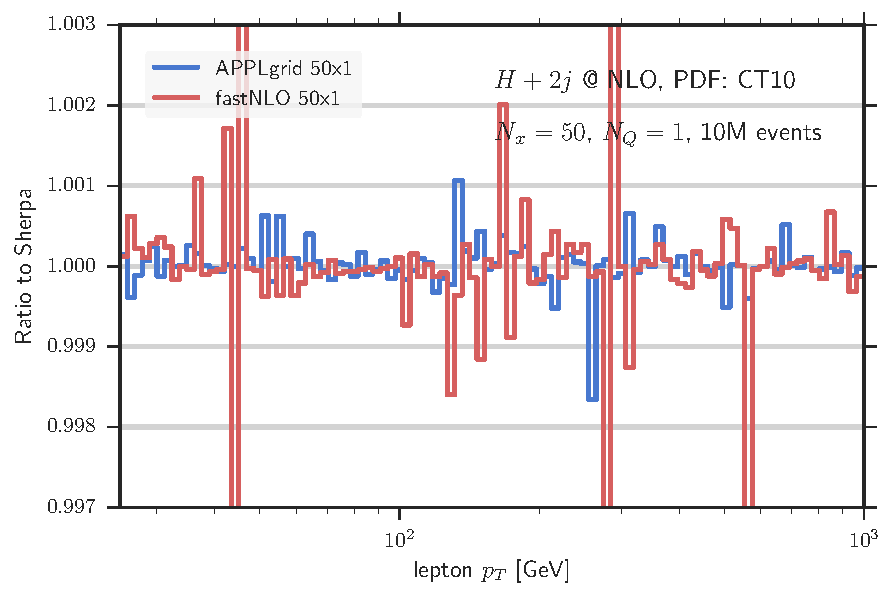
\includegraphics[width=\textwidth]{images/hjjnlo_lpt_50v30.pdf}
\end{subfigure}
\hfill
\begin{subfigure}[]{0.49\textwidth}
	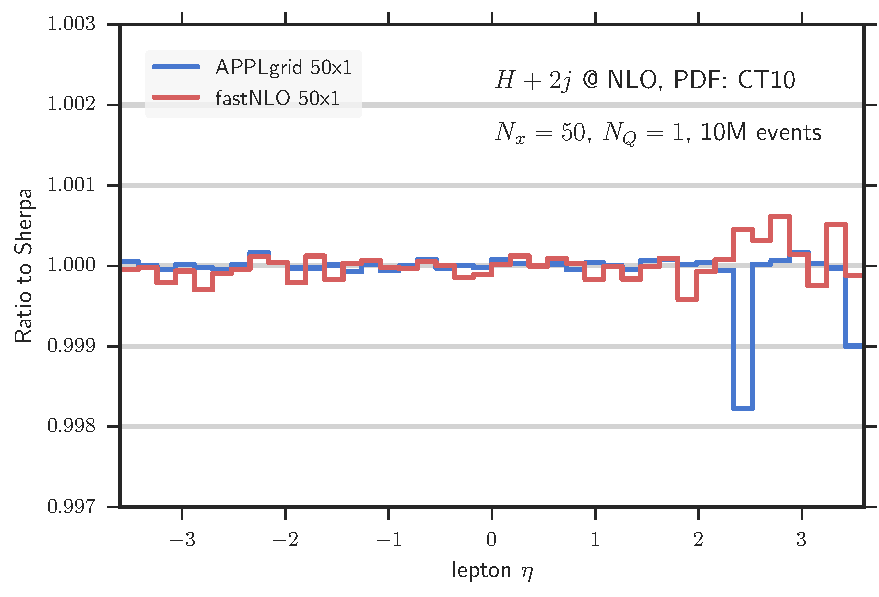
\includegraphics[width=\textwidth]{images/hjjnlo_leta_50v30.pdf}
\end{subfigure}
\caption{H+2j NLO}
\label{fig:hjjnlo_validation}
\end{sidewaysfigure}
%




%
\begin{figure}
\centering
\begin{subfigure}[]{0.49\textwidth}
	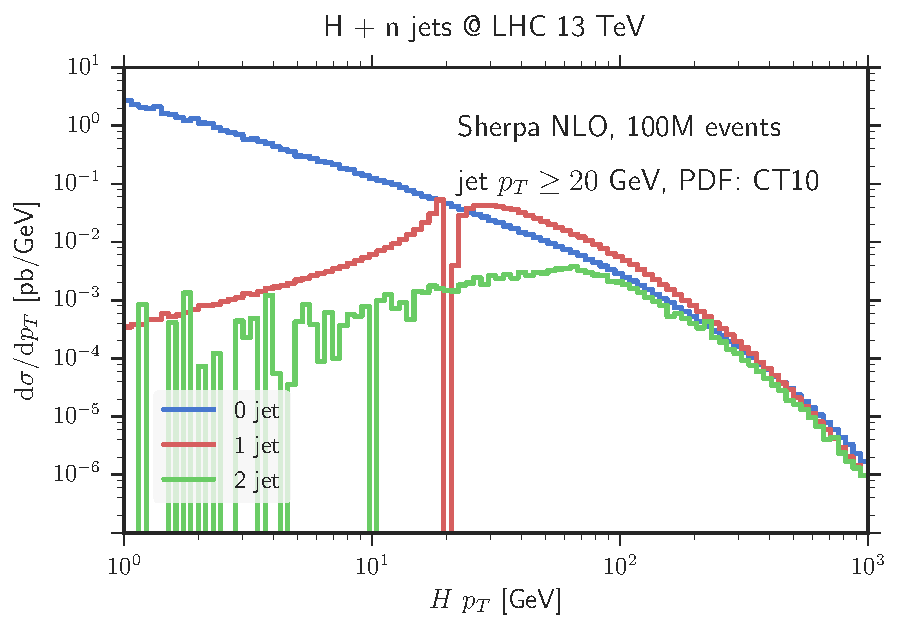
\includegraphics[width=\textwidth]{images/cmp100m_nlo_hpt.pdf}
\end{subfigure}
\hfill
\begin{subfigure}[]{0.49\textwidth}
	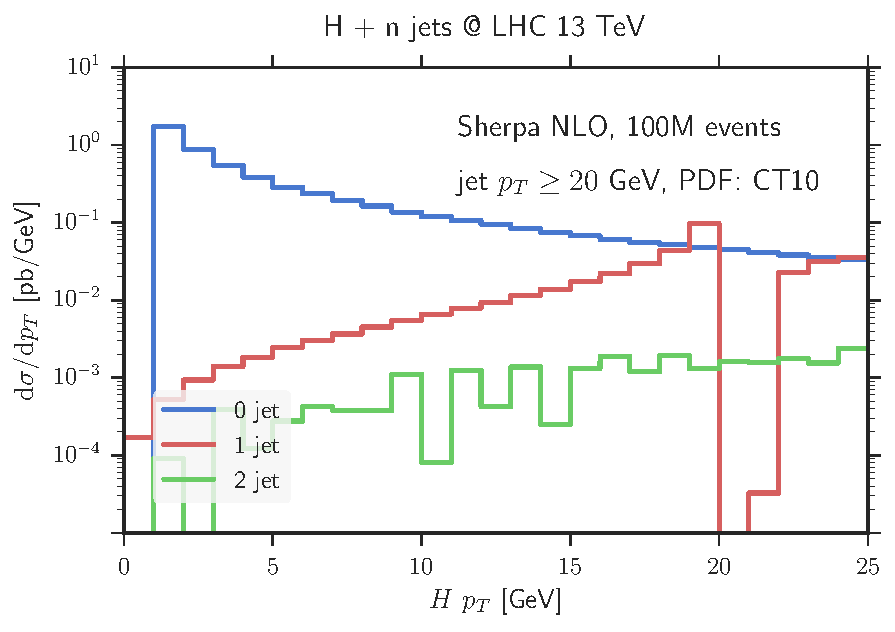
\includegraphics[width=\textwidth]{images/cmp100m_nlo_hptpeak.pdf}
\end{subfigure}
\caption{H pT NLO (0,1,2) jets}
%\label{fig:bla}
\end{figure}
%
\begin{figure}
\centering
\begin{subfigure}[]{0.49\textwidth}
	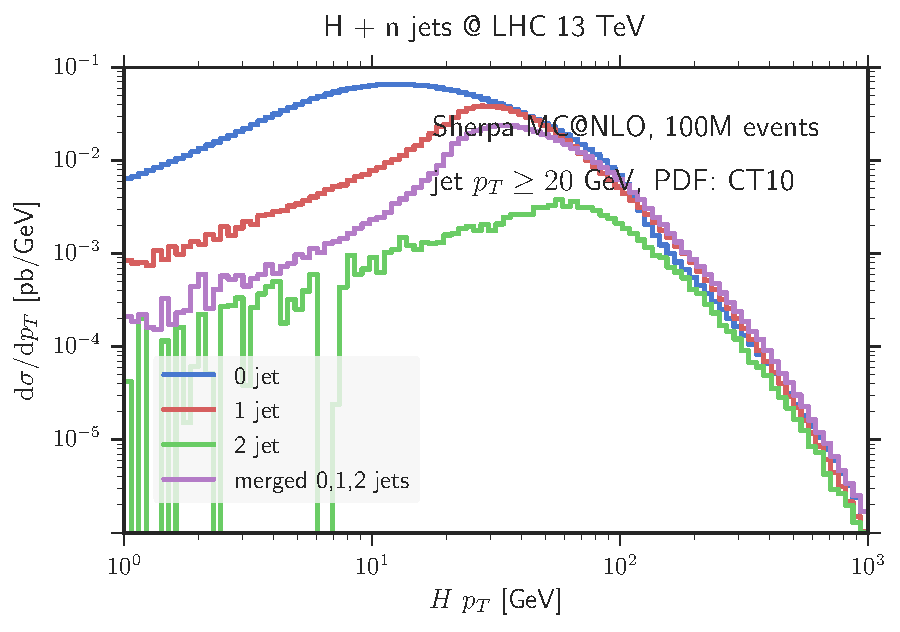
\includegraphics[width=\textwidth]{images/cmp100m_mcatnlo_hpt.pdf}
\end{subfigure}
\hfill
\begin{subfigure}[]{0.49\textwidth}
	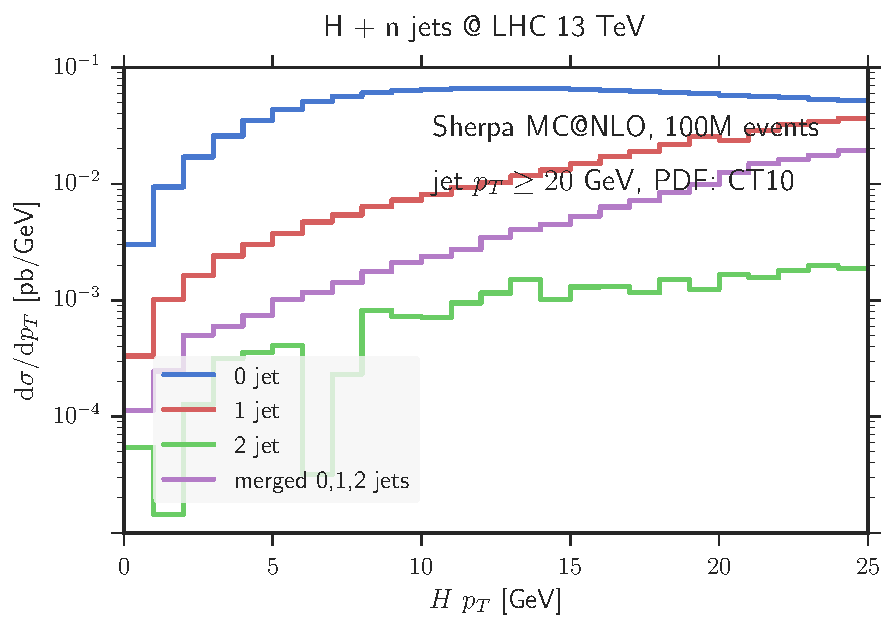
\includegraphics[width=\textwidth]{images/cmp100m_mcatnlo_hptpeak.pdf}
\end{subfigure}
\caption{H pT MCatNLO (0,1,2) jets}
%\label{fig:bla}
\end{figure}
%


%
\begin{figure}
	\centering
	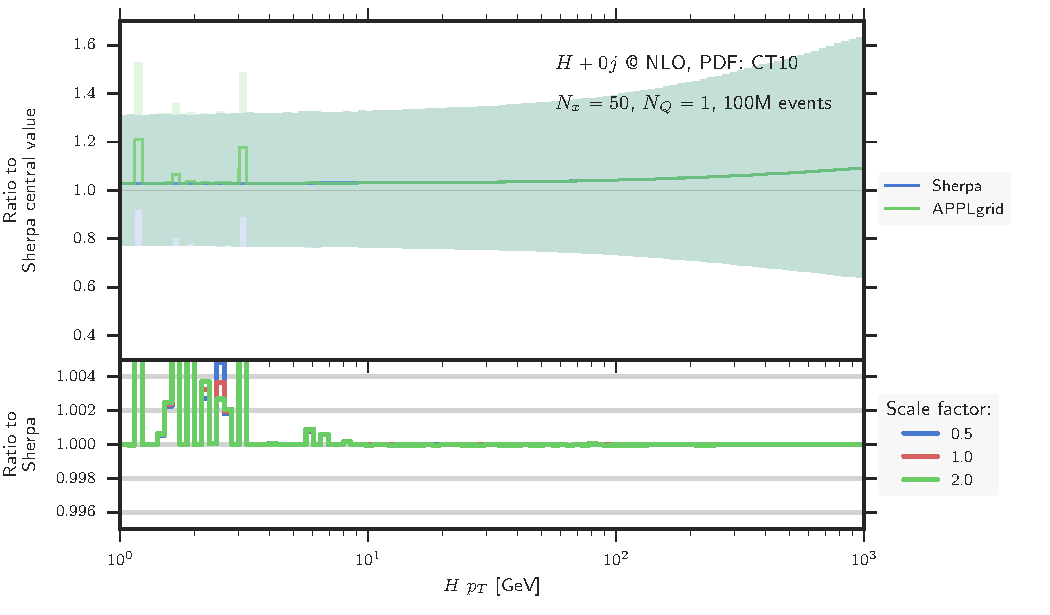
\includegraphics[width=\textwidth]{images/scalesvar_hnlo_appl.pdf}
	\caption{Scale variation appl}
\end{figure}
%
\begin{figure}
	\centering
	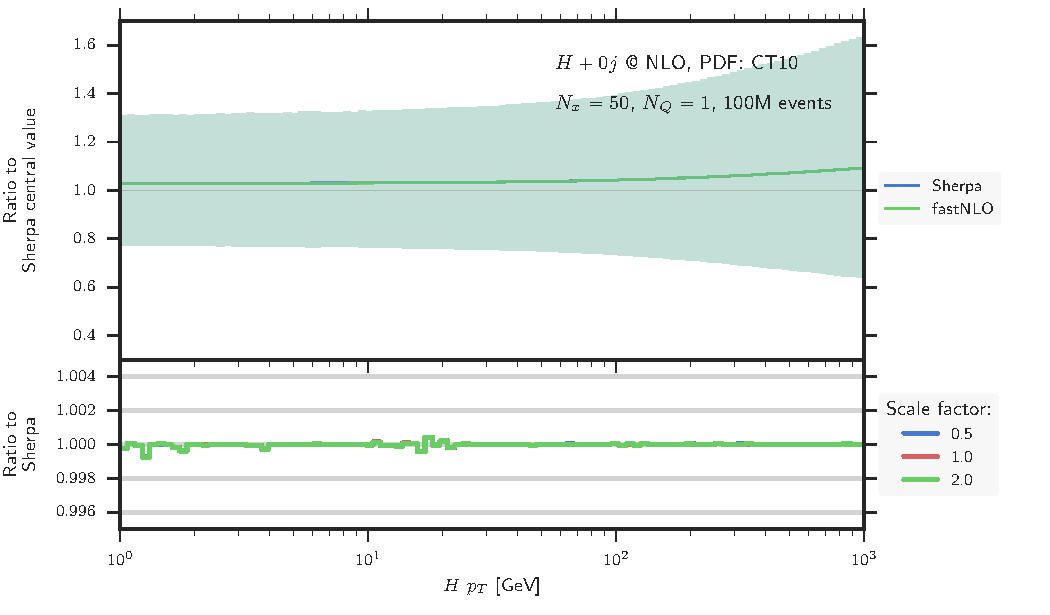
\includegraphics[width=\textwidth]{images/scalesvar_hnlo_fnlo.pdf}
	\caption{Scale variation fnlo}
\end{figure}
%


